\chapter{Hello World}

It is now time for us to start practicing coding skills. In this course, we will be focusing on learning how to program in Java. Java is one of many languages, and eventually you will want to learn others as well. The concepts you learn in this course will make it easier to understand other languages in the future.

Following a long-standing tradition in programming, the first Java program we write will tell the computer to say ``Hello world.''\marginnote{The ``hello world'' program originated in a 1978 book on the C programming language, which is an ancestor of Java.} We will use an application called DrJava to help us create this program.

\section{Starting DrJava}

DrJava is an application that runs on your computer. It knows how to take Java code that you write and use it to tell the computer what to do. Today you'll write your Hello World program in DrJava. First, double click on the DrJava desktop icon to launch the application, as shown in Figure \ref{fig:drjava_launch}.

\begin{figure}
    \centering
    
\begin{tikzpicture}
        \node[scale=5] {Fill this in!};
    \end{tikzpicture}
    \caption{Double click on the DrJava icon to launch the application.}
    \label{fig:drjava_launch}
\end{figure}

Once DrJava opens, you should see a screen like the one in Figure \ref{fig:drjava_fresh}. Most of the DrJava window is taken up by a text box, which is where you will write your code. There are also several menu items organized into a toolbar, which you can use to create new files, open old files, and so on. We will use these menu items today. At the bottom of the screen is where you will eventually tell Java to run your program.

\begin{figure*}
    \centering
    \begin{tikzpicture}
        \node[anchor=south west,inner sep=0] (image) at (0,0) {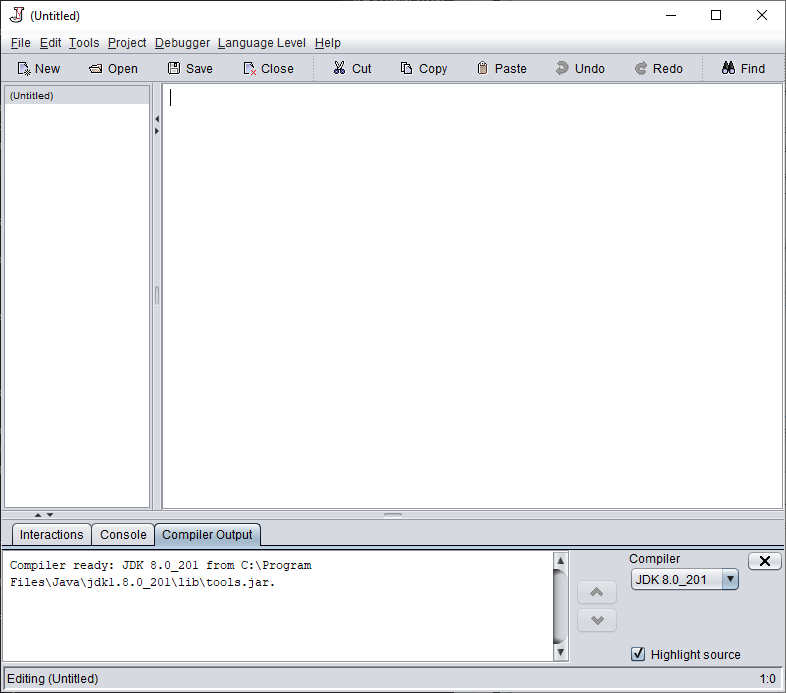
\includegraphics[width=\linewidth]{images/drjava.png}};
        \begin{scope}[x={(image.south east)},y={(image.north west)}]
            \draw[red,ultra thick,->] (.6,.6) node[below] {Text Area} -- (.4,.7);
            \draw[red,ultra thick,->] (.1,.6) node[below] {Open Files} -- (.1,.7);
            \draw[red,ultra thick,->] (.5,.3) node[above] {Java Panel} -- (.5,.2);
            \draw[red,ultra thick,->] (.5,1.05) node[above] {Tool Bar} -- (.5,.93);
        \end{scope}
    \end{tikzpicture}
    \caption{DrJava when it is first launched.}
    \label{fig:drjava_fresh}
\end{figure*}

We will start by making a small change to DrJava which will make it easier for us to discuss our code with each other. Click on the \textbf{Edit} menu, and then at the very bottom of the dropdown, click on \textbf{Preferences}. A new window will open, like the one in Figure \ref{fig:drjava_linenumbers}. On the left panel, click on \textbf{Display Options}. You should see several options appear. Find the checkbox labeled \textbf{Show All Line Numbers}, and check it. Press OK. There should now be numbers along the left-hand side of the text area to make it easy for you to see which line you are writing on. This way, if you want to refer to a line of code, you can say ``look at line 23'' so everyone knows what code you're talking about.  

\begin{figure}
    \centering
    \begin{tikzpicture}
        \node[anchor=south west,inner sep=0] (image) at (0,0) {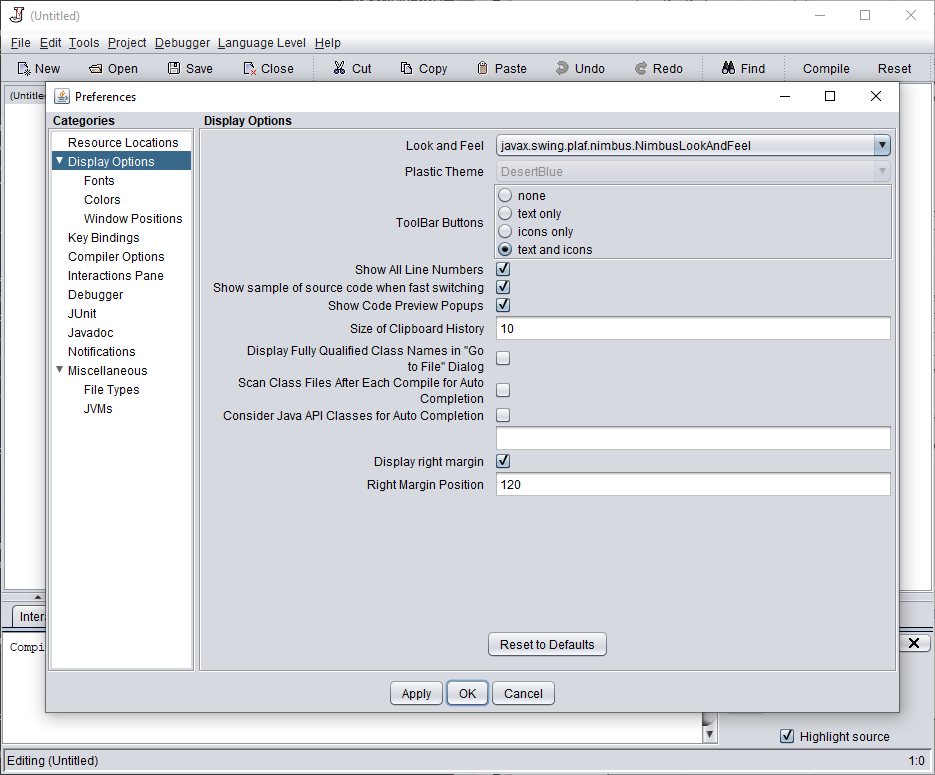
\includegraphics[width=\linewidth]{images/drjava_linenumbers.png}};
        \begin{scope}[x={(image.south east)},y={(image.north west)}]
            \draw[red,ultra thick,->] (.1,1) node[above] {1) Click here} -- (.1,.8);
            \draw[red,ultra thick,->] (.54,1) node[above] {2) Then click here} -- (.54,.67);
        \end{scope}
    \end{tikzpicture}
    \caption{Double click on the DrJava icon to launch the application.}
    \label{fig:drjava_linenumbers}
\end{figure}

\section{Writing your Program}

In Java, every application begins with a class name, and that class must match the filename exactly.

Let's create our first Java program. In the main text area, type the following Java code. We'll learn what this code means shortly.
\begin{code}
class HelloWorld {
    public static void main(String[] args) {
        System.out.println("Hello World!");
    }
}
\end{code}
You'll notice that some of the lines are indented. To produce an indent in your code, use the Tab key on the left side of your keyboard.

Just like Word documents or Excel spreadsheets are stored in files, Java programs are stored in files. When you launched DrJava, it created a new file for you, which is currently called (Untitled). Let's change this name by saving our file. Click on the ``Save'' button in the toolbar above the main text area.

DrJava will open a new window which lets you choose where the file will be saved. First, navigate to your Desktop folder. Once there, follow the instructions in Figure \ref{fig:drjava_saving} to create a new folder called CS103. We will store all of our files for the semester in this folder. 

\begin{figure}[ht]
	\centering
    \begin{tikzpicture}
        \node[anchor=south west,inner sep=0] (image) at (0,0) {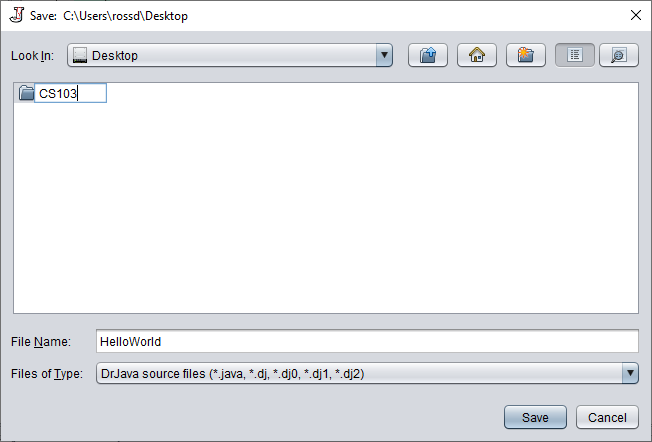
\includegraphics[width=\linewidth]{images/drjava_saving.png}};
        \begin{scope}[x={(image.south east)},y={(image.north west)}]
            \draw[red,ultra thick,->] (.8,1) node[above] {1) Click here} -- (.8,.9);
            \draw[red,ultra thick,->] (.1,1) node[above] {2) Then type CS103} -- (.1,.8);
        \end{scope}
    \end{tikzpicture}
	\caption{Creating a CS103 folder inside your Desktop.}
	\label{fig:drjava_saving}
\end{figure}

Next, double click on CS103 to navigate into the new folder, and then create another folder called ``Chapter\_\thechapter.''

You can now save your file inside the Chapter\_\thechapter\ folder. DrJava will suggest you use the file name \ic{HelloWorld.java}, and you should follow this suggestion. Whenever you have a Java program that starts with \ic{class ABC}, the program must be saved as \ic{ABC.java} for Java to recognize it.\marginnote{This is important to remember!}

\section{Compiling your Program}

Now that we've written some code, we can tell Java to run it. When we ``run'' code, the computer follows the instructions we've laid out in a program and does what you've told it to do. It will take a lot of time to understand the rules Java follows when it runs your code, but you should know from the start that there's nothing mysterious going on. Java will do exactly what you've told it to do, so you just have to make sure that you've given Java the proper instructions.

Running Java code requires a two-step process. The first step is \emph{compilation}. Java compiles the code in your \ic{.java} file into a new file with a \ic{.class} extension. This file contains instructions which are easier for the computer to follow than the instructions as you wrote them. 

You can think of compilation as language translation. Imagine you wrote your code in English, but the computer only speaks Hungarian. The compiler translates your instructions to Hungarian, so that the computer can read the instructions directly.\marginnote{Instead of Hungarian, the compiler actually  outputs ``Java bytecode.''}

To compile your code, click the \textbf{Compile} button towards the right of the toolbar. The compilation should only take a second or two, and then the bottom panel should say \ic{Compilation completed}.

\begin{figure}[ht]
	\centering
    \begin{tikzpicture}
        \node[anchor=south west,inner sep=0] (image) at (0,0) {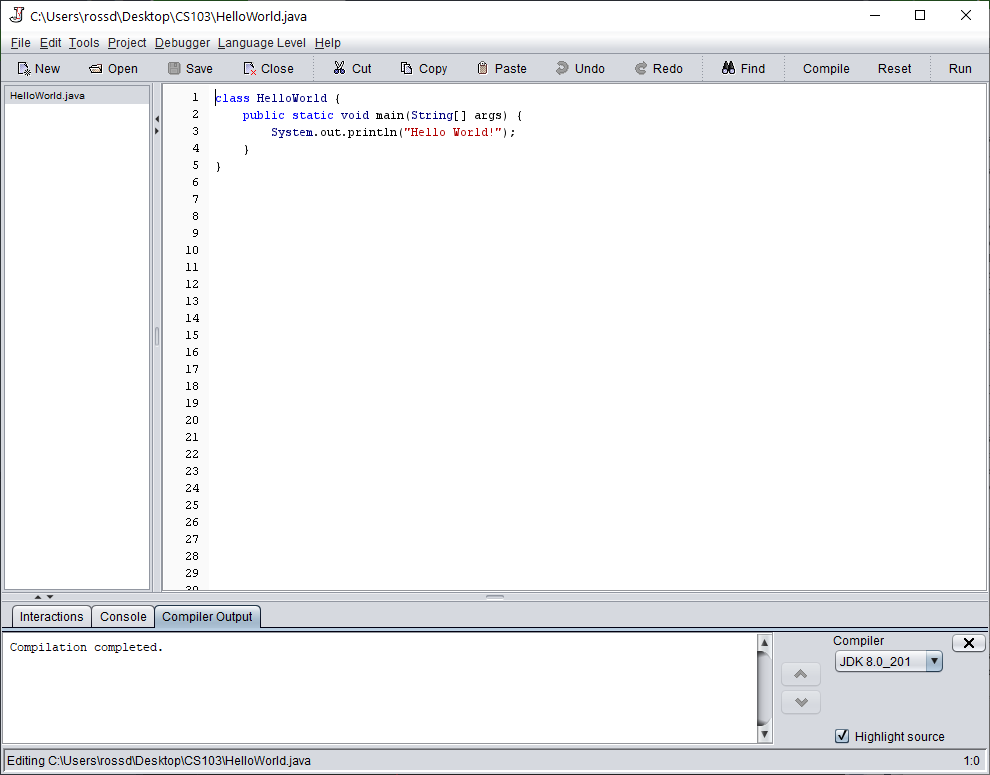
\includegraphics[width=\linewidth]{images/drjava_compiling.png}};
        \begin{scope}[x={(image.south east)},y={(image.north west)}]
            \draw[red,ultra thick,->] (.84,1) node[above] {1) Click here} -- (.84,.92);
            \draw[red,ultra thick,->] (.3,.15) node[right] {2) Then wait for this message} -- (.18,.17);
        \end{scope}
    \end{tikzpicture}
	\caption{Compiling your code in Dr. Java.}
	\label{fig:drjava_compiling}
\end{figure}

\subsection{Compiler Errors}

If there is a problem with your program, you might get an error message when you try compiling. Don't panic! Errors happen all the time, even to experienced programmers. The process of fixing errors is called \emph{debugging}, and it is an incredibly valuable skill. Here we will look at two common errors, and how to fix them. \marginnote{The term ``debugging'' was coined in the 1940s by Admiral Grace Hopper, an early programmer, who had to remove an actual moth from inside an electrical component of her computer!}

Suppose we forgot to include the final curly brace, so that we gave Java the following code:
\begin{code}
class HelloWorld {
    public static void main(String[] args) {
        System.out.println("Hello World!");
    }
\end{code}
If we hit the  ``Compile'' button, then the bottom window should now show an error, with the message \ic{Error: reached end of file while parsing} (see below).
\begin{figure}
	\centering
	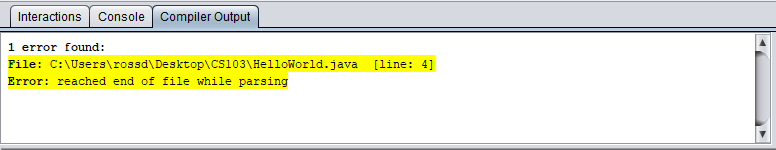
\includegraphics[width=\textwidth]{images/drjava_hello_world_error1.png}
	\caption{If you're missing a curly bracket, Java will complain that it ``reached end of file while parsing.''}
	\label{fig:helloworld:sec:error}
\end{figure}
In general, \ic{Error: reached end of file while parsing} shows up if you did not pair every left curly brace \ic{\{} with a right curly brace \ic{\}}. To fix this error, add the last curly brace \} back in and hit ``Compile'' again.
%Note that in the bottom part of the window, the ``Compiler Output'' tab is selected. This tab is where you can view any messages from compilation.

Another common error is forgetting to end a command with a semicolon, the \ic{;} character. In Java, most lines of code have to end with a semicolon. For example, suppose you write the following code:
\begin{code}
class HelloWorld {
    public static void main(String[] args) {
        System.out.println("Hello World!")
    }
}
\end{code}
Note that Line 4 does not end with a semicolon. If we hit the ``Compile" button, the bottom window will show the error message \ic{Error: ';' expected}.
\begin{figure}
	\centering
	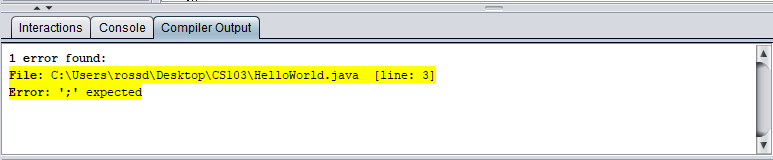
\includegraphics[width=\textwidth]{images/drjava_hello_world_error2.png}
	\caption{If you forget to include a semicolon at the end of a line, Java will tell you that it was expecting a semicolon.}
	\label{fig:helloworld:sec:error2}
\end{figure}

% Let's see another example of a compilation error. Try deleting the semicolon \ic{;} from the program and hit ``Compile.'' The message \ic{Error: ';' expected} arises because the curly brace on line 5 was reached without the semicolon being encountered. In Java, every statement must end in a semicolon. In this case, the print statement on line 4 must end in a semicolon. Add the semicolon back in and recompile the program. Compilation should succeed.

As you progress through the course, you will run into many errors in your programs. This is a normal part of being a programmer. Recognizing different kinds of errors, and knowing how to fix them, are important skills that you will develop in this course.

\section{Running your Program}

Now that the program has been written and compiled, we can run it. We will use DrJava to run our compiled program by clicking the \textbf{Run} button in the toolbar.\marginnote[-2em]{If you don't see the Run button, try dragging the right hand side of your window to make it larger.} 

\begin{figure}[ht]
	\centering
    \begin{tikzpicture}
        \node[anchor=south west,inner sep=0] (image) at (0,0) {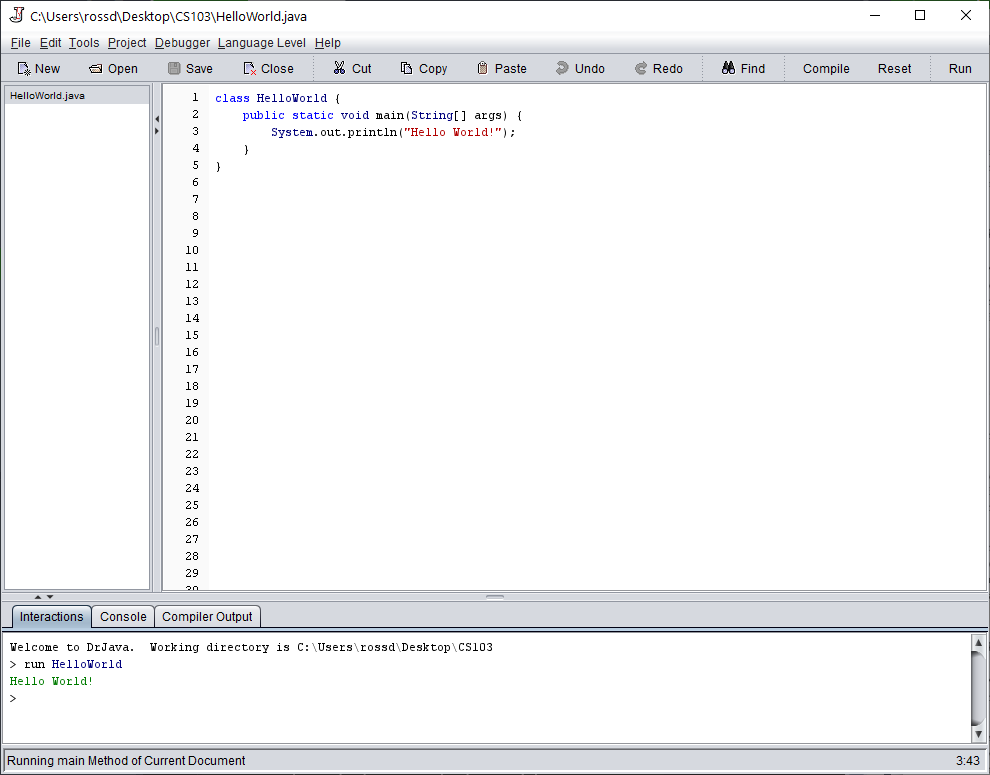
\includegraphics[width=\linewidth]{images/drjava_running.png}};
        \begin{scope}[x={(image.south east)},y={(image.north west)}]
            \draw[red,ultra thick,->] (.97,1) node[above left] {1) Click here} -- (.97,.92);
            \draw[red,ultra thick,->] (.3,.12) node[right] {2) Then Java prints ``Hello World!''} -- (.16,.14);
        \end{scope}
    \end{tikzpicture}
	\caption{Compiling your code in Dr. Java.}
	\label{fig:drjava_compiling}
\end{figure}

After clicking the Run button, you should see the following output in the bottom panel.
\begin{code}
> run HelloWorld 
Hello World!
>
\end{code}

Congratulations! You ran your first Java program.

In the bottom window, the \ic{run HelloWorld} command indicates that you want to run the program \ic{HelloWorld}. The following line shows the output of the program. Programs can have longer output, but this program only printed one line.

When you click the Run button, DrJava opens the \textbf{Interactions} tab of the bottom panel. In the Interactions tab, you can type commands telling Java what programs to run. For instance, you can run your program again by typing \ic{run HelloWorld} and pressing the enter key. You should see the same output printed once again.

\section{How Did it Work?} 

Now let's understand how our \ic{HelloWorld.java} program told Java to print ``Hello World!'' to the screen.

Every line of code that runs in Java must be inside a \emph{class}. In our example, we named the class HelloWorld. A class should always start with an uppercase first letter. Remember, the name of the Java file must match the class name. When saving the file, save it using the class name and add \ic{.java} to the end of the filename. This is why we saved our file for the \ic{HelloWorld} class as \ic{HelloWorld.java}.

\marginnote{General note: Java is case-sensitive, so \ic{HelloWorld} and \ic{helloworld} are distinct. Whenever you name something in Java, make sure you keep the casing consistent!} 

The \ic{main()} ``method'' is required and you will see it in every Java program: 

\begin{code}
public static void main(String[] args)
\end{code}

Any code inside the \ic{main()} method will be executed when we run a program. 

We will learn later what
\ic{public static void} and \ic{String[] args} mean. For now, all you need to know is that every Java program needs a \ic{main} method, and that when we run a Java program, the code within the \ic{main()} method is executed. 

Inside the \ic{main()} method, we use a method provided by Java called \ic{System.out/println()}. This method prints whatever is placed between the open parenthesis \ic{(} and closed parenthesis \ic{)} that follow it.

After every line of Java code inside the \ic{main()} method, a semicolon is required to tell Java that the line is over. Think of a semicolon in Java like a period in English: it tells you where one statement ends and another begins.

\begin{figure}
    \centering
    \begin{tikzpicture}[node distance=0]
        \fill[gray!20] (-4,-3) rectangle (7,4);
        \node[green!50!black,scale=1.3] (method) at (0,0) {\ic{System.out.println}};
        \node[red,scale=1.3,right=of method,inner sep=0] (lparen) {\ic{(}};
        \node[blue,scale=1.3,right=of lparen,inner sep=0] (lq) {\ic{"}};
        \node[orange,scale=1.3,right=of lq,inner sep=0] (hw) {\ic{Hello World!}};
        \node[blue,scale=1.3,right=of hw,inner sep=0] (rq) {\ic{"}};
        \node[red,scale=1.3,right=of rq,inner sep=0] (rparen) {\ic{)}};
        \node[black,scale=1.3,right=of rparen,inner sep=0] (sc) {\ic{;}};
        
        \draw[<-,green!50!black] (method.south) |- ++(-1,-0.5) node[black,left] {Method name};
        \draw[<->,red] (lparen.north) |- ($(lparen.north)!0.5!(rparen.north)+(0,2)$) node[black,above,text width=3cm,align=left] {Parentheses containing method arguments} -| (rparen.north);
        \draw[<->,blue] (lq.south) |- ($(lq.south)!0.5!(rq.south)+(0,-1)$) node[black,below,text width=3cm,align=left] {Quotes containing text to print} -| (rq.south);
        \draw[<-,orange] (hw.north) -- ++(0,1) node[above,black] {Text to print};
        \draw[<-,black] (sc.south) |- ++(-2,-2.5) node[left] {Semicolon to end line};
    \end{tikzpicture}
    \caption{Anatomy of a print statement using \ic{System.out.println}.}
    \label{fig:anatomy_print}
\end{figure}

\section{Experimenting with Hello World}
Now we've successfully written, compiled, and run our first Java program, and have a basic sense of how it is written. Let's try to make our ``Hello World!'' more enthusiastic.

\textbf{Exercise.} Change the \ic{Hello World!} in line 4 to \ic{Hello World!!}. Compile and re-run your program. What does it output now?

Throughout this section, you should practice making changes to your program, recompiling it, and running it again to see the results of your changes.

\subsection{Adding comments to your code}

It is sometimes helpful to provide explanations of what your code is doing. These are known as \emph{comments}. We will look at a few ways to comment your ``Hello World!" program.

Try adding \ic{// print hello} to the end of line 4, so that your line 4 now looks like this:
\begin{code}
        System.out.println("Hello World!!"); // print hello
\end{code}

Now compile and run your program. The behavior should remain unchanged from the previous time you ran the program.

The two forward slashes \ic{//} denote the beginning of an \emph{inline comment}. Comments are ignored by the compiler and do not have any effect on the program's behavior. They are useful for adding explanations or providing information to people that are reading the code. In this case, the comment \ic{print hello} is explaining the purpose of the code on that line.

Now try adding \ic{//} to the beginning of line 4, so that it looks as follows:
\begin{code}
//        System.out.println("Hello World!!"); //print hello
\end{code}
Now compile and run your program. You should find that there is now no output. The two forward slashes that you added turned the whole line into a comment. As far as the compiler is concerned, your program is the same as if the entire line 4 did not exist. This is sometimes called ``commenting out" your code. 

In DrJava, a shortcut for commenting out a line is to hit ''control" and "/" simultaneously. Hitting ''control", "shift", and "/" simultaneously will uncomment code. Try commenting and uncommenting line 4 a few times using the DrJava shortcuts. 

\subsection{Multiple print statements}

Make sure line 4 is not commented out before starting this part. Type the following lines after line 4:
\begin{code}
System.out.println("Hello!"); // print hello again 
System.out.println("Goodbye World!"); // say goodbye
\end{code}
Your code now has \emph{multiple statements}. In particular, you now have three. The first one on line 4 will print
\ic{Hello World!!}, the second one will print \ic{Hello!}, and the third will print \ic{Goodbye World!}.

Your code should look as follows:
\begin{code}
class HelloWorld {
    
    public static void main(String[] args) {
        System.out.println("Hello World!!"); //print hello
        System.out.println("Hello!"); // print hello again
        System.out.println("Goodbye World!"); // say goodbye
    }
    
}
\end{code}
Try compiling it and running it. The output should look as follows:
\begin{code}
Hello World!!
Hello!
Goodbye World!
\end{code}

Note that each of these statements is followed by a semicolon. Deleting any one of these semicolons will result in a compilation error. Try deleting a semicolon and see what happens when you try to compile. 

\subsection{Block comments}

Let's add some description of what we're doing by adding a \emph{block comment}. A block comment begins with \ic{/*} and is ended whenever \ic{*/} is encountered. It may (but does not necessarily need to) span multiple lines. Right before the main method, type a block comment to get the following:
\begin{code}
class HelloWorld {

    /* Main method to print out the following:
         Hello World!!
         Hello!
         Goodbye World!
    */
    public static void main(String[] args) {
        System.out.println("Hello World!!"); //print hello
        System.out.println("Hello!"); // print hello again
        System.out.println("Goodbye World!"); // say goodbye
    }

}
\end{code}
If you compile and run the program now, it should have the same behavior as before, since whatever occurs inside comments does not affect the program's behavior.

Inline comments can be nested inside block comments, so for example, the following program will compile without issue:
\begin{code}
class HelloWorld {

    /* Main method to print out the following:
         Hello World!!
         Hello!
         Goodbye World!
    */
    public static void main(String[] args) {
        /*
        System.out.println("Hello World!!"); //print hello
        System.out.println("Hello!"); // print hello again
        System.out.println("Goodbye World!"); // say goodbye
        */
    }

}
\end{code}
Note that since we have commented out all the code in the main method, this program is actually the same as the following program that we considered earlier:
\begin{code}
class HelloWorld {

    public static void main(String[] args) {
//        System.out.println("Hello World!!"); //print hello
    }

}
\end{code}

\subsection{Understanding whitespace}

Let's now consider the following program that has two print statements and no comments:
\begin{code}
class HelloWorld {

    public static void main(String[] args) {
        System.out.println("Hello!");
        System.out.println("Goodbye!");
    }

}
\end{code}
Try compiling and running the program. Note the output. What happens when we remove the linebreaks and spaces between each pair of print statements?
Try removing them to get the following:
\begin{code}
class HelloWorld {

    public static void main(String[] args) {
        System.out.println("Hello!");System.out.println("Goodbye!");
    }

}
\end{code}
Now compile and run the program. What happens?
The behavior should still be such that it prints the same output:
\begin{code}
Hello!
Goodbye!
\end{code}
\emph{Whitespace} such as linebreaks and spaces do not have any meaning in Java. While spaces are necessary to separate things like \ic{class} and \ic{HelloWorld} or \ic{String[]} and \ic{args}
so that Java can distinguish between them, spaces are otherwise unimportant. Line breaks have no significance at all in a Java program except to denote when an inline comment should end.

That being said, whitespace should be used to make your code more legible. Although you can write all your Java programs on a single line, it is considered very bad style!
For demonstrative purposes, here the original Hello World Java program all on two lines:
\begin{code}
class HelloWorld{public static void main(String[] args)
    {System.out.println("Hello World!");}}
\end{code}
Try removing whitespaces in your code, and then compile and run it. It should still print \ic{Hello World!} as its output. You can even get rid of all the spacing after the close parenthesis \ic{)} to get the whole program on a single line--it just doesn't fit on the page if it's all on one line in these notes!
